\section{目的}
依講義 PDF 78--80 頁重建 Lab 19 的電源 IR drop 與 decoupling capacitor 比較，回答電流峰值與電容成本。

\section{Spec 對照}
S 表示已執行模擬檢查，D 表示分析與討論。

\small\begin{longtable}{p{.46\linewidth}p{.30\linewidth}p{.15\linewidth}}\toprule
要求與 PDF 頁碼 & 對應 deck／檢查 & 狀態 \\ \midrule\endhead
圖19.1四級負載、兩個1歐姆電阻（78,80） & D01/C0 & S \\
觀察內外電源、地與R1/R2電流（78,80） & D01; printed traces & S \\
10pF/100pF/1nF比較（79--80） & D01/C1--3 & S \\
電流峰值、代價與使用時機（80） & Results/discussion & S+D \\
\bottomrule\end{longtable}\normalsize


\section{電路與設計推導}
四級 inverter 的倍數依序為 30、60、180、540，單位 $W_p/W_n/L=3.6/1.8/0.25\,\mu$m。外部電源與內部 VDD、內部地與全域地之間各串 1 $\Omega$；最後一級另接 10 fF 到內部地。去耦電容接在內部 VDD 與內部地間，不是接外部理想電源。未加電容以 $10^{-21}$ F 近似。
\[\Delta V_R=IR,\qquad i_C=C\,d(V_{DD,int}-V_{GND,int})/dt.\]
這是集中 RC 的電源模型，沒有由版圖萃取金屬線或封裝電感。

\section{模擬設定}
模型由使用者於本機另行提供；採 1 V、27 $^\circ$C 的教學適配條件，不把講義舊製程的 2.5 V 數值視為本次通過門檻。使用 PrimeSim HSPICE S-2021.09、\texttt{accurate}、\texttt{runlvl=5}，由實際 \texttt{.print/.measure} 數據繪圖。每個 \texttt{.alter} 重設全部基準參數與溫度。所有案例皆完成，無 error 或 failed 量測；這不代表完全沒有模型或收斂提示。公開 netlist 僅保留 \texttt{* MODEL\_SETUP\_REQUIRED} 註解，不附模型路徑。完整數據位於該 lab 的 \texttt{results/}，大型資料依 deck 分檔，由 \texttt{simulation\_data.json} 索引。本 lab 為一份 deck、四案例。輸入 0--1 V、50 ps 邊緣，1 ns 延遲，2 ns 高準位、4 ns 週期；模擬 20 ns，最大步距 2 ps。摘要以 4--20 ns 的同一觀察窗量測。

\section{結果與規格檢查}
\begin{center}\small\begin{tabular}{lrrrrr}\toprule
C & $V_{rail,min}$ & $\Delta V_{rail,pp}$ & $I_{R1,pk}$ & $I_{R2,pk}$ & $P_{avg}$ \\ \midrule
0 & 0.93453 & 63.350 & 32.734 & 32.738 & 9.923 \\
10 pF & 0.93486 & 62.301 & 32.570 & 32.573 & 9.930 \\
100 pF & 0.94510 & 50.913 & 27.447 & 27.449 & 9.975 \\
1 nF & 0.96779 & 23.425 & 17.507 & 17.283 & 9.520 \\
\bottomrule\end{tabular}\end{center}
表中最小 rail 電壓單位 V，rail 峰峰值單位 mV，電流單位 mA、平均功率單位 mW。無去耦時最小差動電源約 0.93453 V；1 nF 時約 0.96779 V。R1 峰值從 32.734 mA 降至 17.507 mA；R2 也有相同趨勢。10 pF 改善很小，顯示電容需相對於負載切換電荷才有意義。
\begin{figure}[htbp]\centering
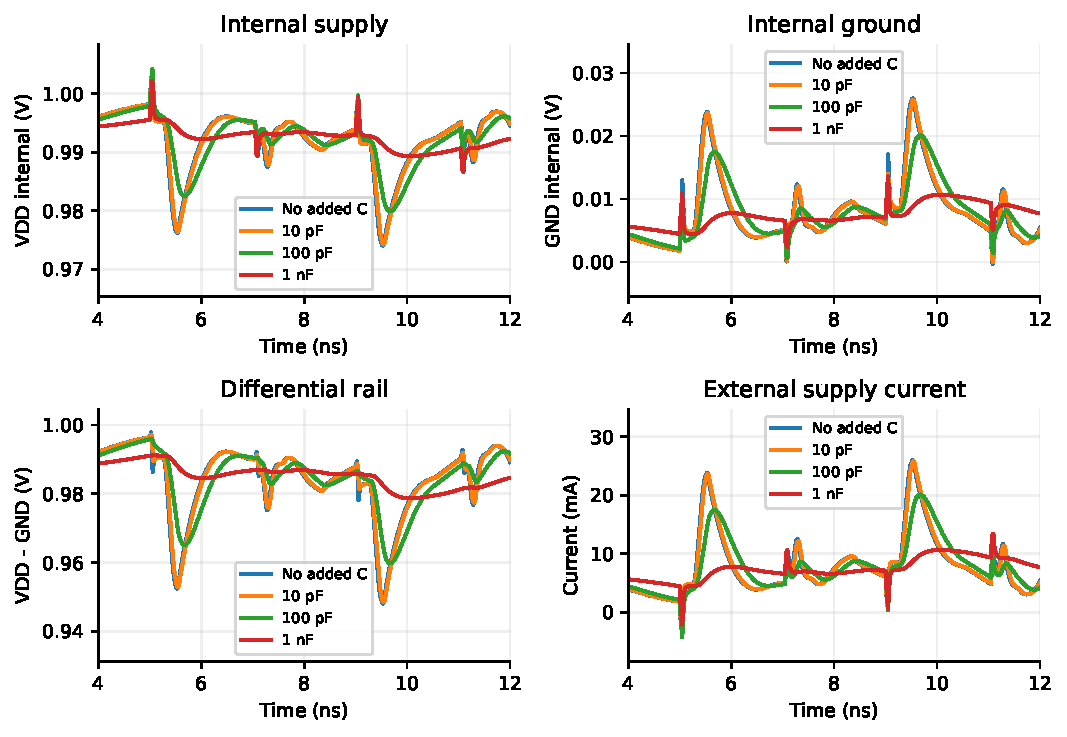
\includegraphics[width=\linewidth]{figures/supply_decoupling.pdf}
\caption{實際電源、地、差動電源與供應電流；放大顯示 4--12 ns，摘要使用完整 4--20 ns。}
\end{figure}


\section{討論}
電容在快速切換時就近供應／吸收電荷，外部電阻支路的瞬時電流較平滑，因此峰值壓降降低；它不會消除平均 DC 的 IR drop。電容越大，瞬態供電越穩，但佔用實體面積，增加充電與啟動時間，且真實電容有漏電、ESR/ESL 與製造限制。此處沒有用理想電容數字推估實體面積。

是否需要去耦應由允許的電源雜訊、最大同步切換電流與電源阻抗決定。可先改善電源線阻抗或錯開切換；對快速且局部的大電流負載再評估電容。表中的平均功率只是有限觀察窗，不能從較小的供應峰值推論能量消耗一定下降；電容充放電與初始條件也會影響平均值。

\section{結論}
四種電容條件與兩條電源支路皆已實際模擬。1 nF 明顯減小差動 rail 波動，但不等於電源電位完全固定，也不構成實體電源完整性簽核。
